\chapter{Model checking}
\section{Introduzione}
Le \textbf{logiche temporali} sono una famiglia di logiche matematiche che
permette di esprimere proprietà che cambiano nel tempo.

Quando si analizzano sistemi reattivi (quindi concorrenti) allora non vale più
il ragionamento di avere uno stato precedente e uno stato successivo che varia nel
tempo.

Sono stati introdotti diversi modelli per modellare i sistemi concorrenti, ora
si introdurranno nuove tecniche di analisi.

Esempio produttore consumatore in Java. Esempio concorrente e gli elementi sono
indipendenti quindi si devono sincronizzare quando si accede al buffer. Vogliamo
garantire la correttezza del programma:
\begin{itemize}
    \item Ogni oggetto deve essere prima prodotto
    \item Ogni oggetto non può essere consumato più di una volta
    \item Il sistema non raggiunge mai uno stato di \textbf{deadlock}
\end{itemize}
Le reti di Petri ci permettono di controllare se si mantiene la mutua esclusione,
ovvero che non esista una  marcatura in cui entrambi i processi non possono essere
negli stati $c_1$ e $c_2$. Noi vorremmo modellare il blocco di uno dei due
processi se uno si trova nella zona critica.

Vogliamo quindi un modello per verificare se sono valide delle proprietà di
interesse e se il modello rappresenta effettivamente il sistema.
\begin{definizione}
    Un sistema è \textbf{reattivo} se è un sistema concorrente, distribuito e
    asincrono.
\end{definizione}
Una sottoclasse dei sistemi reattivi sono quelli sincroni con un clock ma è una
semplificazione.

I sistemi reattivi non obbediscono più al paradigma input-computazione output,
rendendo quindi impossibile utilizzare le triple di Hoare per dimostrare la
correttezza di un programma. Possiamo sempre riutilizzare la logica di hoare per
dimostrare alcuni pezzi ma dovremmo usare un modo per unire i risultati.

Al posto delle triple di Hoare, utilizzeremo delle \textbf{asserzioni}, ovvero
delle frasi conteneti elementi temporali che descrivono il comportamento del sistema.
\begin{esempio}
    Se è stato spedito un messaggio allora questo prima o poi verrà ricevuto dal
    destinatario
\end{esempio}
\begin{esempio}
    Se si accende una spia di allarme allora questa sarà accesa fino a quando non
    si spegne il dispositivo
\end{esempio}
Vediamo ora come possiamo procedere nell'analisi dei sistemi concorrenti. Il
problema che vogliamo risolvere è quello di stabilire se un sistema reattivo è
corretto. Per fare ciò, seguiremo il seguente schema:
\begin{enumerate}
    \item Si esprime il criterio di correttezza come una formula di un opportuno
          linguaggio logico.
    \item Si modella il sistema nella forma di un sistema di transizioni.
    \item Si valuta se la formula è vera nel sistema di transizioni. (algoritmi)
\end{enumerate}
\begin{definizione}[\textbf{Sistema di transizioni}]
    Un \textbf{sistema di transizioni} è definito da:
    \begin{equation}
        A=(Q,T)
    \end{equation}
    dove:
    \begin{itemize}
        \item $Q$ insieme degli stati (non per forza finito)
        \item $T\subseteq Q\times Q$ insiemi di transizioni di stato
    \end{itemize}
\end{definizione}
\begin{definizione}[\textbf{Cammino}]
    Definiriremo un \textbf{cammino} come una sequeza di stati $\pi$ dove
    \begin{equation}
        \pi = q_0q_1\dots q_n \ (q_i,q_{i+1})\in T \ \forall i
    \end{equation}
    (combacia con la definizione di cammino su grafi).
\end{definizione}
\begin{definizione}[\textbf{Suffisso}]
    Definiriremo un \textbf{suffisso} di ordine $i$ per un cammino $\pi$ è il
    cammino che inizia da uno stato di indice $i$.
    \begin{equation}
        \pi^{(i)} = q_iq_{i+1}\dots q_n
    \end{equation}
\end{definizione}
\begin{definizione}[\textbf{Cammino massimale}]
    Definiriremo un \textbf{cammino massimale} se il cammino è finito e non può
    essere esteso, cioè solo quando il cammino raggiunge uno stato che non ha
    transizioni uscenti. (cammino massimale finito)
\end{definizione}
Il cammino massimale è infinito quando non si ha uno stato pozzo.
\begin{nota}
    Ogni suffisso di un cammino massimale è a sua volta un cammino massimale.
\end{nota}
Posso rappresentare un cammino espandendo la definizione delle espressioni regolari,
aggiungendo $^\omega$ per rappresentare una sequenza infinita. Bisogna prestare
particolare attenzione al fatto che $\omega \neq \ast$, inaftti $\ast$ mi rappresenta
una sequenza arbitraria di valori.
\begin{nota}
    Posso esprimere un cammino come un suffisso di ordine 0.
\end{nota}
\section{Logica Temporale Lineare}
Definiamo la \textbf{sintassi} partendo dalle proposizioni atomiche:
\begin{equation}
    AP=\{ p_1,p_2,\dots,p_i,\dots \}
\end{equation}
composte dalle asserzioni considerate vere a prescindere.
\begin{esempio}
    Il messaggio è stato spedito, la spia di allarme è accesa
\end{esempio}
Definiamo anche le formule ben formate $FBF_{LTL}$:
\begin{itemize}
    \item Ogni proposizione atomica è una formula ben formata.
    \item $\top$ e $\bot$ sono formule ben formate.
    \item se $\alpha,\beta\in FBF$ allora $\alpha\lor \beta,\lnot \alpha \in FBF$
          (da queste si derivano tutti i connettivi logici).
    \item Operatori temporali siano $\alpha$ e $\beta$ formule ben formate, allora
          anche:
          \begin{itemize}
              \item $X\alpha$ "next $\alpha$" nel prossimo stato $\alpha$ è vera.
              \item $F\alpha$ "future $\alpha$" prima o poi $\alpha$ sarà vera.
              \item $G\alpha$ "globally $\alpha$" $\alpha$ è sempre vera.
              \item $\alpha\mathbb{U}\beta$ "until $\alpha$" $\alpha$ è vera fino
                    a quando $\beta$ diventa vera.
          \end{itemize}
          sono formule ben formate.
\end{itemize}
Per definire la sintassi utilizzeremo i \textbf{Modelli di Kripke} che prendono
i sistemi di transizione e li arricchiscono associando a ogni stato $q \in Q$
l'insieme delle proposizioni atomiche che sono vere in $q$. Quindi possiamo
definire:
\begin{equation}
    I \ : \ Q \rightarrow 2 ^{AP}
\end{equation}
dove $2^{AP}$ è l'insieme delle parti di $AP$. Un modello di Kripke sarà definito
come:
\begin{equation}
    A=(Q,T,I)
\end{equation}
Con un modello di Kripke possiamo identificare per uno stato quali sono le
proposizioni atomiche vere e per capire se le FBF sono vere allora dovrò analizzare
i cammini che partono dallo stato in esame.

Vediamo ora come associare una semantica alle formule ben formate. Per fare ciò
procediamo in due fasi:
\begin{enumerate}
    \item Definiamo un criterio per stabilire se una formula $\alpha$ è vera in
          un cammino massimale $\pi$.
    \item Diciamo che la formula è vera rispetto a uno stato $q$ se è vera in
          tutti i cammini massimali che partono da $q$.
\end{enumerate}
Fissiamo quindi un cammino generico $\pi$ e $\alpha$ una formula ben formata allora
\begin{equation}
    \pi \vDash \alpha \iff \ \text{significa che} \ \alpha \ \text{è vera nel cammino}
    \ \pi
\end{equation}
Definiremo la relazione $\vDash$ per induzione.
\begin{definizione}
    Supponiamo che $\alpha$ e $\beta$
    siano due formule ben formate e $p$ una preposizione atomica:
    \begin{itemize}
        \item $\pi \vDash \top$
        \item $\pi \not\vDash \bot$
        \item $\pi \vDash p \iff p\in I(q_0)$
        \item $\pi \vDash \lnot \alpha \iff \pi \not\vDash \alpha$
        \item $\pi \vDash  \alpha \lor \beta \iff (\pi \vDash \alpha)\lor (\pi \vDash
                  \beta) $
        \item Operatori temporali: supponiamo $\beta, \gamma \in FBF$
              \begin{itemize}
                  \item $\pi\vDash X\beta \iff \pi^{(1)}\vDash \beta$
                  \item $\pi\vDash F\beta \iff \exists i \in \mathbb{N}:\pi^{(i)}
                            \vDash \beta$
                  \item $\pi\vDash G\beta \iff \forall i \in \mathbb{N}:\pi^{(i)}
                            \vDash \beta$
                  \item $\pi \vDash \beta \mathbb{U} \gamma \iff$:
                        \begin{itemize}
                            \item $\exists i \in \mathbb{N}$ tale che $\pi^{(i)}\vDash
                                      \gamma$ cioè $\pi\vDash F\gamma$
                            \item $\forall h, 0\le h < i, \pi^{(h)}\vDash \beta$
                        \end{itemize}
                        Se $\gamma$ è vera fin da subito, quindi $i=0$ allora $\beta$
                        è superfluo
              \end{itemize}
    \end{itemize}
\end{definizione}
\begin{esempio}
    Ecco alcuni esempi:
    \begin{itemize}
        \item $FG\alpha$: esprime che da un certo momento in poi $\alpha$ sarà
              invariante, se $\alpha = \perp$ allo stato iniziale ma $FG\alpha = \top$
              vale dallo stato iniziale allora significa che non si tornerà più
              in quello stato.
        \item $GF\alpha$: $\alpha$ è vera in un numero infinito di stati
        \item $G\lnot (cs_1\land cs_2)$: mutua esclusione se $cs_1$ indica il
              processo è nella sezione critica, viceversa $cs_2$.
        \item $G(req \implies XF ack)$:
        \item $G(req \implies (req U ack))$: se c'è la richiesta allora la richiesta
              è pendente fino a quando si ha un'ack. Si differenzia da quella
              precedente dal momento che la richiesta deve rimanere fino a quando
              non si manda l'ack.
        \item $G(req \implies ((req\land \lnot ack) U (\lnot req \land ack)))$:
              si chiede di non rispondere all'inizio e dopo la risposta la richiesta
              viene cancellata
    \end{itemize}
\end{esempio}
\begin{esempio}
    Consideriamo la seguente rete di Petri, la quale rappresenta due processi che
    vogliono accedere ad una risorsa condivisa.
    \begin{figure}
        \centering
        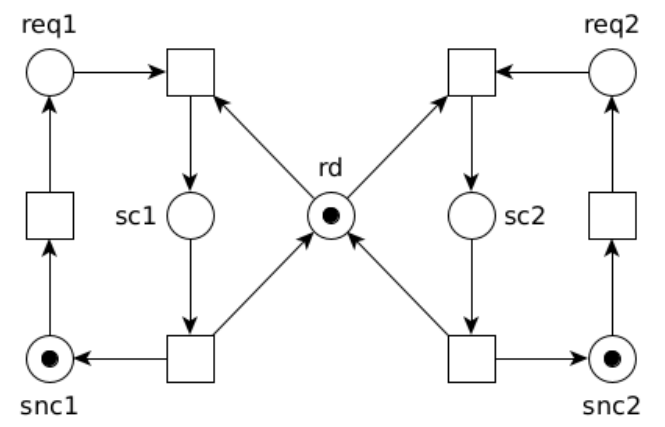
\includegraphics[width=0.5\textwidth]{img/model/retePetriEsempio.png}
        \caption{Rete di Petri per il model checking}
    \end{figure}
    Questa rete è composta da:
    \begin{itemize}
        \item $rd$ la risorsa disponibile.
        \item $sc1$ e $sc2$ le due sezioni critiche.
        \item $snc1$ e $snc2$ le due sezioni non critiche.
        \item $req1$ e $req2$ le due richieste di usare la risorsa.
    \end{itemize}
    Per poter applicare le tecniche di model checking dobbiamo trasformare questa
    rete in un modello di Kripke. Per farlo dobbiamo definire gli stati e le
    transizioni. Una possibile soluzione è quella di calcolare il grafo dei casi
    (o grafo di raggiungibilità) della rete di Petri ed assegnare ad ogni nodo
    un insieme di proposizioni atomiche che sono vere in quel nodo.

    Possiamo quindi definire il grafo dei casi dove per semplicità utilizziamo il
    nodo $1$ come stato iniziale:
    \begin{figure}[!ht]
        \centering
        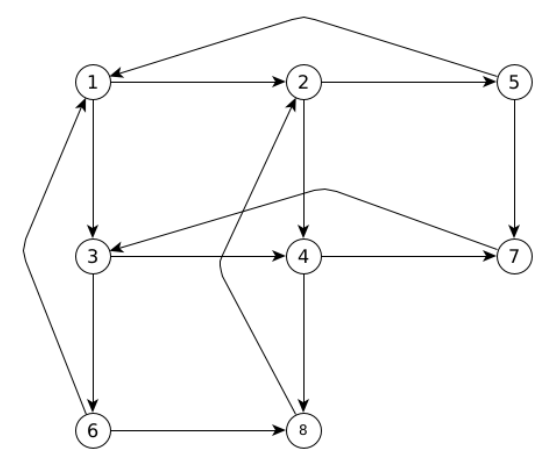
\includegraphics[width=0.5\textwidth]{img/model/GrafoDeiCasi.png}
        \caption{Grafo dei casi della rete di Petri}
    \end{figure}
    dove ogni nodo è rappresentato da:
    \begin{itemize}
        \item $1=\{rd,snc1,snc2\}$
        \item $2=\{rd,req1,snc2\}$
        \item $3=\{rd,snc1,req2\}$
        \item $4=\{rd,req1,req2\}$
        \item $5=\{sc1, snc2\}$
        \item $6=\{snc1,sc2\}$
        \item $7=\{sc1, req 2\}$
        \item $8=\{req1,sc2\}$
    \end{itemize}
    Una volta cstruita la struttura, definiamo delle formule che vogliamo siano
    vere per la situazione in analisi. Studiamo quindi:
    \begin{itemize}
        \item $G\neq (sc_1\land sc_2)$: esprime che non si può raggiungere
              uno stato in cui entrambi i processi sono nella sezione critica.
        \item $G\,(req1\implies F\,sc1)$: esprime che se il processo 1 fa richiesta
              allora prima o poi entrerà nella sezione critica.
    \end{itemize}
    Per verificare le formule dovremmo considerare tutti i cammini massimali che
    partono dallo stato 1 e verificare che le formule siano valide in tutti i
    cammini. Tuttavia, questo caso è complesso e i possibili cammini massimali
    sono potenzialmente infiniti.

    Una via più facile è, osservando che dallo stato si possono raggiungere tutti
    gli altri stati, scorrere la tabella delle formule vere in ciascun stato e
    osservare che in nessun stato è vera la formule $sc_1 \land sc_2$.

    Per la seconda formula non possiamo più applicare questa strategia, ma possiamo
    cercare di confutare la formula: basta trovare un cammino massimale che non
    soddisfi la formula.

    In ogni caso questa seconda formula non è valida in quando potrei avere il
    cammino $(1)(2,4,8)^\omega$ in cui anche il secondo processo fa richiesta e
    ci entra. Posso entrare in un loop in cui solamente il processo due prende
    ogni volta la risorsa quindi la formula non è valida in quel cammino massimale.

    Possiamo comunque trovare cammini in cui vale, come $(1,3,6)^\omega$, in
    quanto in quei tre stati $req1$ è sempre falsa.

    Una possibile soluzione è quella di aggiungere un nuovo stato $9$, duplicando
    lo stato $4$ in modo da implementare un meccanismo di \textbf{turno} in cui
    i processi si alternano nell'uso della risorsa.
\end{esempio}
Come per tutte le logiche, anche per la logica temporale si può definire una
equivalenza tra formule.
\begin{definizione}[\textbf{Equivalenza tra formule}]
    Possiamo definire l'\textbf{equivalenza tra formule} come:
    \begin{equation}
        \alpha \equiv \beta \iff \forall \pi : ( \pi \vDash \alpha \iff \pi \vDash \beta)
    \end{equation}
\end{definizione}
\begin{esempio}
    Vediamo ora alcuni esempi di equivalenza tra formule:
    \begin{itemize}
        \item $F\alpha \equiv \alpha \lor XF\alpha$ se prima o poi $\alpha$ sarà
              vera, allora o è vera in questo stato oppure dal prssimo stato
              $\alpha$ sarà prima o poi vera.
        \item $G\alpha \equiv \alpha \land XG\alpha$ se $\alpha$ Se è sempre vera,
              allora è vera in questo stato e dal prossimo stato sarà sempre vera.
        \item $\alpha U \beta \equiv \beta \lor (\alpha \land X(\alpha U \beta))$
              se $\beta$ è vera non ci interessa altro, oppure $\alpha$ è vera e
              dal prossimo stato $\alpha$ sarà vera fino a quando $\beta$ diventa
              vera.
        \item $FGF \alpha \equiv GF\alpha$ se prima o poi $\alpha$ sarà vera, allora
              da un certo momento in poi $\alpha$ sarà sempre vera.
        \item $GFG\alpha \equiv FG\alpha$ se $\alpha$ è sempre vera, allora da un
              certo momento in poi $\alpha$ sarà sempre vera.
        \item $\top U\alpha \equiv F\alpha$: questo significa che l'operatore
              $F$ non è essenziale
        \item $\lnot F \lnot \alpha\equiv G\alpha$: questo significa che $G$ può
              essere definito a partire da $F$ quindi l'insieme minimale di
              operazioni sono $\{X,U\}$. Questo insieme minimale non è unico.
    \end{itemize}
\end{esempio}
Le equivalenze spesso sfruttano la ricorsione dal momento che si basano su sistemi
di transizione.

Le equivalenze logiche permettono di definire degli \textbf{operatori derivati},
per velocizzare la scrittura delle formule. Alcuni esempi di operatori derivati
sono:
\begin{itemize}
    \item \textbf{Until debole}: $\alpha W \beta \equiv G\alpha \lor
              (\alpha U \beta)$ con questo operatore si può esprimere la proprietà
          in cui $\alpha$ è sempre vera oppure $\alpha$ è vera fino a quando
          $\beta$ diventa vera.
    \item \textbf{Release}: $\alpha R \beta$ per cui
          \begin{equation}
              \pi\vDash\alpha R \beta \iff \forall k\ge 0:(\pi^{(k)}\vDash \beta\lor
              \exists h<k:\pi^{(h)}\vDash \alpha)
          \end{equation}
          In sostanza o $\beta$ è sempre vera oppure $\beta$ potrà essere falsa
          solo quando $\alpha$ diventa vera. Definito in questo modo allora si può dire
          \begin{equation}
              \alpha R \beta \equiv \beta W (\alpha \land \beta)
          \end{equation}
\end{itemize}
\begin{definizione}[\textbf{Insieme di operatori minimale}]
    L'insieme degli operatori è detto \textbf{minimale} se ogni altro
    operatore può essere definito a partire da questi. Un esempio di inisieme di
    operatori minimale per le logiche temporlai è $\{X,U\}$.
\end{definizione}
Attenzione all'uso della negazione nelle formule LTL, cosa significa "non è vero
$F\alpha$"?  Significa che $\exists$ un cammino per cui non vale $F\alpha$.  Mentre
$\lnot F\alpha \equiv G\lnot \alpha$ quindi $\lnot F\alpha$ non è la negazione di
$F\alpha$. Qundi dobbiamo stare attenti ai quantificatori universali nascosti.

Negli esercizi sulla logica temporale ci possono essere diverse risposte giuste.
Ecco degli esercizi sulla logica temporale lineare.
\begin{esempio}
    Traduci questa frase:
    \begin{center}
        Chi ruba, presto o tardi finirà in galera.
    \end{center}
    possiamo considerare 2 proposizioni atomiche:
    \begin{itemize}
        \item $hr$: ho rubato
        \item $c$: sono in carcere
    \end{itemize}
    Si può riformulare la frase come una legge, quindi come una cosa che vale sempre,
    portandoci ad utilizzare l'operatore $G$. In aggiunta, possiamo riformularla
    in un modo che ha una semantica più vicina alla semantica degli operatori logici
    \begin{center}
        Se rubi, in futuro finirai in galera.
    \end{center}
    Si può tradurre in
    \begin{equation}
        G(hr\implies XF \ c)
    \end{equation}
    Utilizziamo l'operatore $X$ per evitare che nel momento in cui rubo allora
    subito finisco in galera.

    Possiamo provare a tradurre la frase
    \begin{center}
        Solo chi ruba finirà in galera.
    \end{center}
    Quindi si può tradurre
    \begin{equation}
        \lnot c \ W \ hr \equiv G(c \iff hr)
    \end{equation}
\end{esempio}
\begin{esempio}
    Traduci questa frase:
    \begin{center}
        Chi ruba finirà in carcere, ma solo dopo avere parlato con un avvocato.
    \end{center}
    si aggiunge anche la proposizione atomica: "ho parlato con un avvocato"
    \begin{equation}
        G(hr\implies (XF \ c \land (\lnot c \ U \ pa)))
    \end{equation}
    Si potrebbe pensare che $XF \ c$ si possa escludere ma in realtà no perché
    $U$ porta a dire che dopo aver parlato con un avvocato non vuol dire che $c$
    diventi vera.
\end{esempio}
\begin{esempio}
    Traduci questa frase:
    \begin{center}
        Se la cabina è in movimento verso l'alto, si trova all'altezza del secondo
        piano, ed è stato premuto il pulsante interno di richiesta del quinto piano,
        allora la cabina non cambierà direzione fino a quando avrà raggiunto il
        quinto piano.
    \end{center}
    si specificano le proposizioni atomiche:
    \begin{itemize}
        \item $su$: "la cabina sta salendo"
        \item $p_i$: "cabina all'altezza del piano $i$"
        \item $r_i$: "pulsante interno del piano $i$ è stato premuto"
    \end{itemize}

    \begin{equation}
        G((su \land p_2 \land r_5)\implies(su \ U \ p_5))
    \end{equation}
\end{esempio}
La logica temporale che abbiamo studiato fino a questo momento (LTL) permette di
esprimere diverse prprietà dei sistemi reattivi, ma ha dei limiti, infatti non
permette di esprimere proprietà del tipo:
\begin{center}
    \emph{``esiste un cammino in cui $\alpha$''}
\end{center}
Il problema è che queste proprietà sono utili, per risolvere questa mancanza
introduciamo una nuova logica. Questa logica può essere interpretata attraverso
il concetto di \textbf{albero di computazione}.
\begin{definizione}
    Un \textbf{albero di computazione} è una struttura che mi permette di
    rappresentare le possibili computazioni di un sistema di transizioni
    etichettato.

    I cammini che partono dalla radice di questo albero sono definiti come
    \textbf{computazioni} del sistema.
\end{definizione}
\begin{nota}
    Spesso si vuole esprime le possibili computazioni di un sistema allora possiamo
    costruire un albero (simile all'\textbf{unfolding} per le reti di petri) che
    rappresenta la computazione rispetto gli stati globali.

    L'albero può essere construito in modo induttivo:
    \begin{itemize}
        \item Si sceglie lo stato iniziale
        \item Se si hanno transizioni verso altri stati allora li aggiungo come
              prossimi nodi
        \item Così via ricorsivamente, se ci sono archi all'indietro allora
              si ricrea un altro nodo in avanti.
    \end{itemize}
    Nel caso fosse ciclico allora sarà infinito, se abbiamo stati in deadlock allora
    il nodo sarà pozzo.
\end{nota}
\section{Computation Tree Logic - CTL}
Possiamo definire ora la logica CTL (\textbf{Computation Tree Logic}), ovvero
una logica temporale che si basa sugli alberi di computazione.

Definiremo la \textbf{sintassi} attraverso le $FbF_{CTL}$.
\begin{itemize}
    \item $\forall p \in AP, p\in FbF_{CTL}$ con $AP =\left\{p1,p2,\dots\right\}$
          insieme delle preposizioni atomiche.
    \item $\forall \alpha, \beta \in FbF_{CTL}$
          \begin{itemize}
              \item $\lnot\alpha, \alpha \lor \beta \in FbF_{CTL}$
              \item $AX \ \alpha, EX \ \alpha \in FbF_{CTL}$ per ogni / esiste
                    un cammino dallo stato corrente tale che nello stato prossimo
                    vale $\alpha$
              \item $AF \ \alpha, EF \ \alpha \in FbF_{CTL}$ per ogni / esiste
                    un cammino dallo stato corrente tale che prima o poi vale $\alpha$
              \item $AG \ \alpha, EG \ \alpha \in FbF_{CTL}$ per ogni / esiste
                    un cammino dallo stato corrente tale che vale sempre $\alpha$
              \item $A(\alpha \ U \ \beta), E(\alpha \ U \ \beta)\in FbF_{CTL}$
                    per ogni / esiste un cammino dallo stato corrente tale che
                    $\alpha$ è vera fino a quando $\beta$ non diventa vera.
                    ($\beta$ deve per forza diventare vera)
          \end{itemize}
\end{itemize}
In particolare abbiamo aggiunto $A$ e $E$ i quali rappresentano due quantificatori
sui cammini. Essi sono definiti come segue:
\begin{itemize}
    \item $A$ è il quantificatore universale e si interpreta come per ogni cammino.
    \item $E$ è il quantificatore esistenziale e si interpreta come esiste un
          cammino tale che.
\end{itemize}
Quindi ogni occorrenza di un operatore temporale sarà associata ad un quantificatore
$A=\forall$ e $E= \exists$ che si applica ai cammini.
\begin{esempio}
    Traduciamo
    \begin{center}
        Dopo l'accensione della spia, sarà sempre possibile riportare il sistema
        allo stato iniziale.
    \end{center}
    Definiamo:
    \begin{itemize}
        \item $s$: la spia è accesa
        \item $init$: il sistema si trova nello stato iniziale
    \end{itemize}
    \begin{equation}
        AG(s\implies AX \ EF \ init)
    \end{equation}
\end{esempio}
\begin{esempio} [Esercizio d'esame]
    Dato il sistema di transizione riportato in figura \ref{fig:esercizioEsame},
    vogliamo verificare la seguente proprietà:
    \begin{itemize}
        \item $AF \ q$
        \item $AG (EF (p \lor q))$, $GF(p \lor q)$
        \item $EX (EX \ r)$, $XX \ r$
        \item $AG (AF \ q)$
    \end{itemize}
    \begin{figure}[!ht]
        \centering
        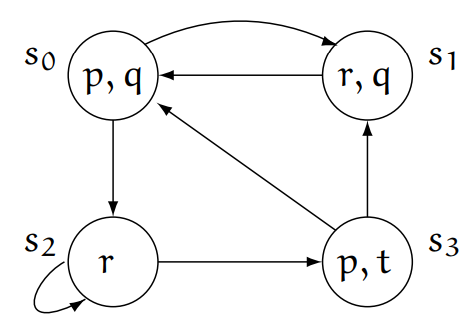
\includegraphics[width=0.5\textwidth]{img/model/esercizioEsame.png}
        \caption{Sistema di transizione}
        \label{fig:esercizioEsame}
    \end{figure}
    Vediamo ora come risolvere i vari punti:
    \begin{itemize}
        \item $AF \ q$: in questo caso conviene suddividere la formula ed
              analizzare gli elementi semplici, come $F$ e $q$. A questo punto
              controlliamo per ogni stato dove vale $q$, in questi stati, per
              come abbiamo definito $F$ la formula risulta vera. Quindi negli
              stati $s_0$ e $s_1$ la formula è vera. Successivamente verifico se
              sui cammini che partono dagli altri stati $q$ diventa vera. Questo
              è vero per il cammino che parte da $S_3$, ma non per quello che parte
              da $s_2$, dal momento che in quest'ultimo stato è presente un
              cappio quindi può non andare mai in $s_3$.
        \item $GF(p \lor q)$: avendo questa formula non basta analizzare dove
              valgono $p$ o $q$ perchè abbiamo $G$ quindi dobbiamo controllare
              anche che per tutti gli stati successivi $p$ o $q$ siano vere.
              Partendo dallo stato $s_0$ la formula è falsa in quanto si arriva
              in $s_2$ dove nessuno delle due sono vere. $s_2,s_3$ vero ma anche
              $s_1$ è falsa. %% TODO: controllare. Non è sempre falsa perché posso arrivare sempre in $s_2$ e restarci per il cappio?
        \item $AG (EF (p \lor q))$: è vera per tutti gli stati perché esiste
              sempre un cammino con una deviazione in cui vale $p \lor q$.
        \item $XX \ r$: non è vera in $s_0$ perché abbiamo trovato un cammino
              per cui non è vera $s_0\to s_1\to s_0$. Mentre $s_1$ è verificata.
        \item $EX (EX \ r)$: è vera in $s_0$ perché abbiamo trovato un cammino
              per cui è vera $s_0\to s_2\to s_2$ e a noi ne basta una sola.
        \item $AG (AF \ q)$: non vale in $s_2$ perché possiamo rimanere
              all'infinito, Mentre negli altri è sempre vera.
    \end{itemize}
\end{esempio}
\begin{nota}[\textbf{Non siamo sicuri sia vera}]
    Ricorda che per la semantica della logica $LTL$ allora tutte le $FbF_{LTL}$
    sono equivalenti alle $FbF_{CTL}$ che hanno l'operatore $A$ e viceversa.
\end{nota}
Anche per questa logica definiremo l'equivalenza logica.
\begin{definizione}[\textbf{Formule equivalenti}]
    Due formule $\alpha$ e $\beta$ sono equivalenti, indicato come $\alpha \equiv
        \beta$, se e solo se:
    \begin{equation}
        \forall \pi \land \forall \models : (\pi \models \alpha \iff \pi \models
        \beta)
    \end{equation}
\end{definizione}
In entrambe le logice, LTL e CTL, possiamo esprimere le seguenti proprietà:
\begin{itemize}
    \item \textbf{Invariante}: si possono avere delle formule sempre vere:
          \begin{equation}
              AG\lnot p \equiv G\lnot p
          \end{equation}
    \item \textbf{Rieattiva}: il valore logico di una formula implica la veridicità
          di un'altra:
          \begin{equation}
              AG (p\implies AF \ q) \equiv G(p\implies F \ q)
          \end{equation}
\end{itemize}
Le due logiche non hanno la stessa potenza espressiva ma nessuna delle due è più
espressiva rispetto all'altra. Infatti per esempio la logica CTL può esprimera
la seguente proprietà (\textbf{reset property}):
\begin{center}
    Da ogni stato raggiungibile in ogni cammino è sempre possibile raggiungere
    uno stato nel quale vale $p$
\end{center}
Esprimibile secondo la seguente formula $AG \ EF \ p$, per cui non esiste una formula
LTL che possa esprimere la proprietà.

Al contrario la logica LTL può esprimere la seguente proprietà
\begin{center}
    In ogni cammino, prima o poi si raggiungerò uno stato a partire dal quale $p$
    rimane sempre vera.
\end{center}
Esprimibile secondo la seguente formula $F \ G \ p$, per cui non esiste una formula
CTL che possa esprimere la proprietà.

Quindi CTL e LTL sono delle logiche temporali che hanno poteri espressivi diversi,
ovvero esistono formule che possono essere espresse in una logica ma non nell'altra.

Per ovvieare a questo problema si definisce l'estensione di CTL (CTL$^\ast$),
in particolare, si rimuove dalla logica CTL il vincolo di avere un quantificatore
che precede ogni operatore temporale.

Lo svantaggio di questa logica è che richiede un maggiore sforzo computazionale
per dimostrare le proprietà, sarà quindi importante decidere quale logica usare.
\begin{figure}[!ht]
    \centering
    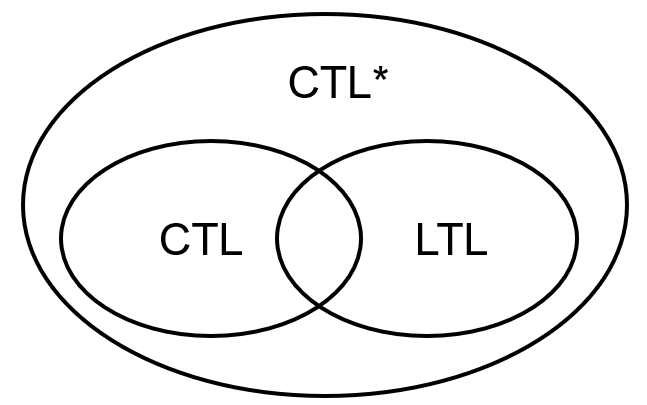
\includegraphics[width=0.5\textwidth]{img/model/logicheTemprali.png}
    \caption{Relazione tra le logiche temporali}
\end{figure}